\documentclass[class=book, crop=false, oneside]{standalone}
\usepackage[subpreambles=true]{standalone}

\usepackage{../../style}
\usepackage{../../set-citations}

\graphicspath{{./assets/images/}}

% arara: pdflatex: { synctex: yes, shell: yes }
% arara: latexmk: { clean: partial }
\begin{document}
\chapter{La gerarchia di memoria}\begin{fquote}[Burks, Goldstine, Von Neumann][1946]Idealmente si desidererebbe una memoria indefinitamente grande, in cui ogni particolare parola risulti immediatamente disponibile.
\end{fquote}

\section{Introduzione}
Sottolineare quanto il concetto di memoria sia importante e necessario nei dispositivi elettronici del giorno d'oggi risulta abbastanza scontato. D'altra parte, viene fatta subito una precisazione: non esiste un'unica soluzione che permette di ottenere la memoria "perfetta"; esistono infatti diverse implementazioni, ognuna con i suoi compromessi, che variano per costo, prestazioni e capacità.

\subsection*{Qualche definizione}
Possiamo distinguere principalmente due tipologie di memoria in base alla modalità di accesso:
\begin{itemize}
	\item \emph{memoria indirizzata direttamente} (memoria principale, memoria cache):
	\begin{itemize}
		\item è volatile, ossia il suo contenuto viene perso se viene spento il calcolatore;
		\item è limitata per capacità dallo spazio di indirizzamento definito dall'architettura del processore;
		\item i dati contenuti nella memoria principale sono disponibili in qualsiasi momento;
	\end{itemize}
	\item \emph{memoria indirizzata indirettamente} (memoria periferica):
	\begin{itemize}
		\item è di tipo permanente, ossia mantiene il suo contenuto anche senza alimentazione;
		\item ha uno spazio di indirizzamento software che non dipende dall'architettura del processore;
		\item i dati contenuti nella memoria periferica devono essere trasferiti alla memoria principale prima di essere utilizzati (solitamente questo processo viene mediato dal software, tipicamente il sistema operativo);
	\end{itemize}
\end{itemize}

A seguire un elenco di definizioni che utilizzeremo in seguito.
\begin{itemize}
	\item \emph{Tempo di accesso}: è il tempo richiesto per \emph{una} operazione di lettura / scrittura nella memoria;
	\item \emph{Tempo di ciclo}: è il tempo che intercorre fra l'inizio di due istruzioni consecutive; è composto dal tempo di accesso sommato al tempo di transito del dato con cui si lavora;
	\item \emph{Latenza}: è il tempo di acceso ad una singola parola; indica quanto il processore dovrebbe poter aspettare un dato dalla memoria nel caso peggiore;
	\item \emph{Velocità o "banda"}: velocità di trasferimento massima in FPM\footnote{Fast Page Mode, per la definizione si guardi la sezione~\ref{sec:FPM}.}; oltre ad essere importante per le operazioni FPM che sono legate all'utilizzo della memoria cache interne ai processori, è significativa per le operazioni in DMA (ossia quando un dispositivo periferico viene collegato alla memoria senza passare per il processore);
	\item \emph{Accesso casuale}: è quella modalità di accesso in cui non vi è alcun ordine o relazione fra i dati memorizzati; è tipico delle memorie a semiconduttori;
	\item \emph{Accesso sequenziale}: è quella modalità che presuppone lo scorrimento ordinato di un blocco di dati per accedere ad un suo dato; il tempo d'accesso dipende dalla posizione fisica del dato nel supporto (tipicamente nastri e dischi);
	\item \emph{RAM} (\emph{Random Access Memory}): è una memoria dotata di accesso casuale che permette scrittura e lettura; viene implementata attraverso semiconduttori;
	\item \emph{ROM} (\emph{Read Only Memory}): è una memoria a semiconduttori che prevede solo un accesso in lettura; esistono implementazioni sia attraverso accesso casuale che sequenziale
\end{itemize}

\section{La memoria principale}
\subsection{Le RAM}
Con la seguente immagine descriviamo come avviene la connessione logica fra memoria RAM e CPU:
\begin{figure}[H]
	\centering
	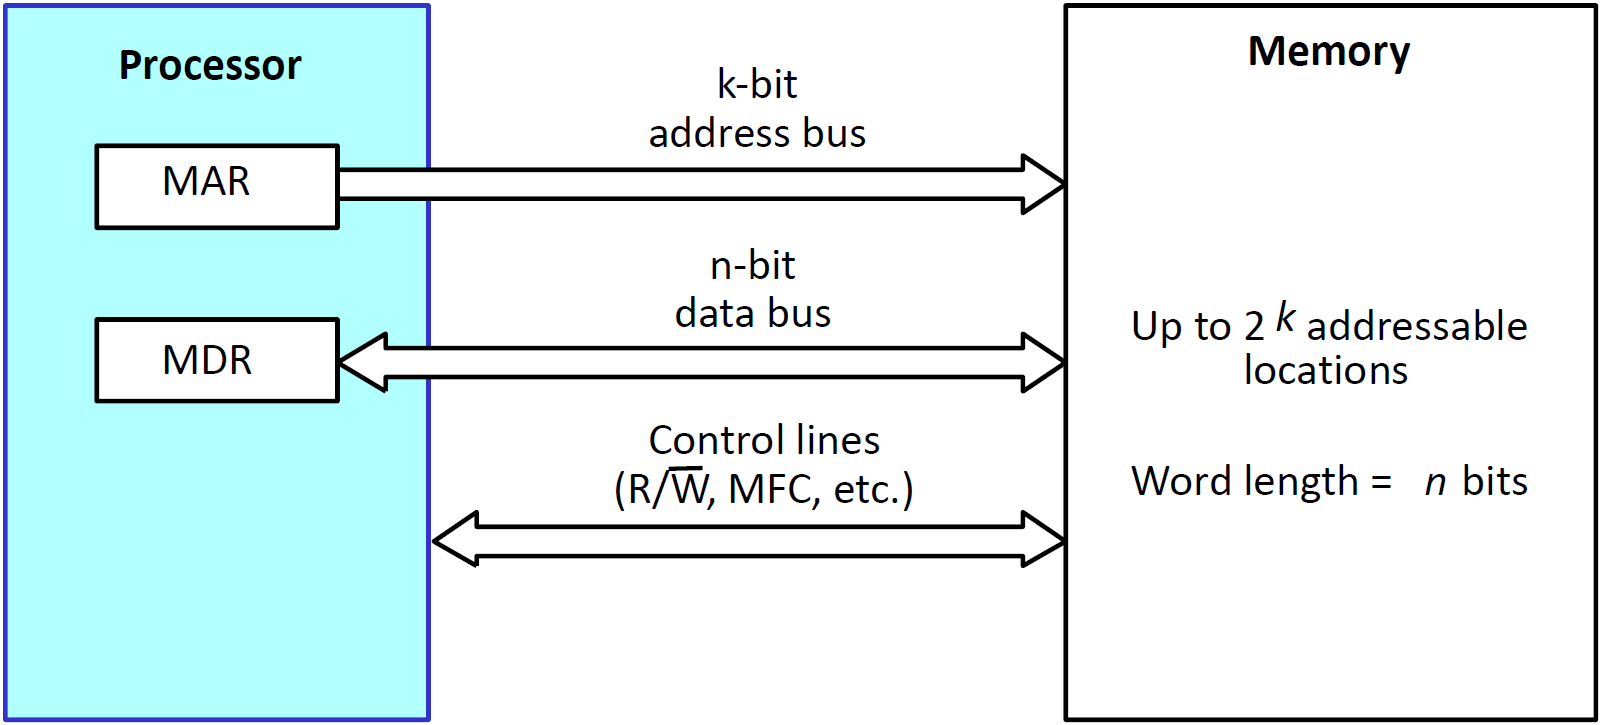
\includegraphics[width=0.7\textwidth,keepaspectratio]{relazione_cpu_ram.png}
	\caption{Modello della relazioni logiche fra CPU e RAM}
\end{figure}
Esistono principalmente 3 bus che permettono di far comunicare il processore con la memoria:
\begin{itemize}
	\item \emph{MAR} (\emph{Memory Address Register}): è un bus a \(k\) bit, dove \(2^k\) sono il numero massimo di indirizzi accessibili direttamente in memoria. Dal punto di vista pratico contiene l'indirizzo del dato (o istruzione) che si vuole caricare o scrivere;
	\item \emph{MDR} (\emph{Memory Data Register}): è un bus a \(n\) bit, dove \(n\) è la lunghezza delle word nella memoria. Dal punto di vista pratico contiene il dato (o l'istruzione) che si vuole caricare o scrivere;
	\item \emph{bus di controllo:} è un bus che contiene vari codici di controllo che permettono di pilotare le relazioni fra memoria e CPU. Alcune linee di controllo sono: il bit \emph{MFC} (\emph{Memory Function Completed}) che permette di stabilire se l'operazione di lettura o scrittura è stata completata e il bit \emph{\(\textrm{R/}\overline{W}\)}, che distingue se si sta eseguendo un'operazione di lettura o scrittura.
\end{itemize}
Si noti che il \emph{MAR} è stato rappresentato da una freccia unidirezionale: dopo aver definito l'indirizzo di memoria su cui lavorare, infatti il processore non si aspetta il risultato. Vengono gestiti diversamente i bus di controllo e \emph{MDR}, i quali sono rappresentati con una freccia bidirezionale, in quanto sia la memoria che la CPU possono occupare il ruolo di mittente del messaggio.

Una memoria \emph{RAM} a semiconduttori principalmente immagazzina singoli bit, memorizzati normalmente in gruppi di byte e/o word per motivi di efficienza. La memoria non necessariamente deve essere strutturata monoliticamente: è possibile che sia suddivisa in diversi blocchi, al fine di favorire il parallelismo; si noti comunque che la dimensione complessiva della memoria non varia se presa in un unico blocco o se separata. Si ricorda che l'organizzazione di una memoria influenza il numero di pin di I/O del circuito integrato: più saranno, più aumenterà il costo.

\subsubsection{Organizzazione dei bit in un banco di memoria 16x8}
\begin{figure}[H]
	\centering
	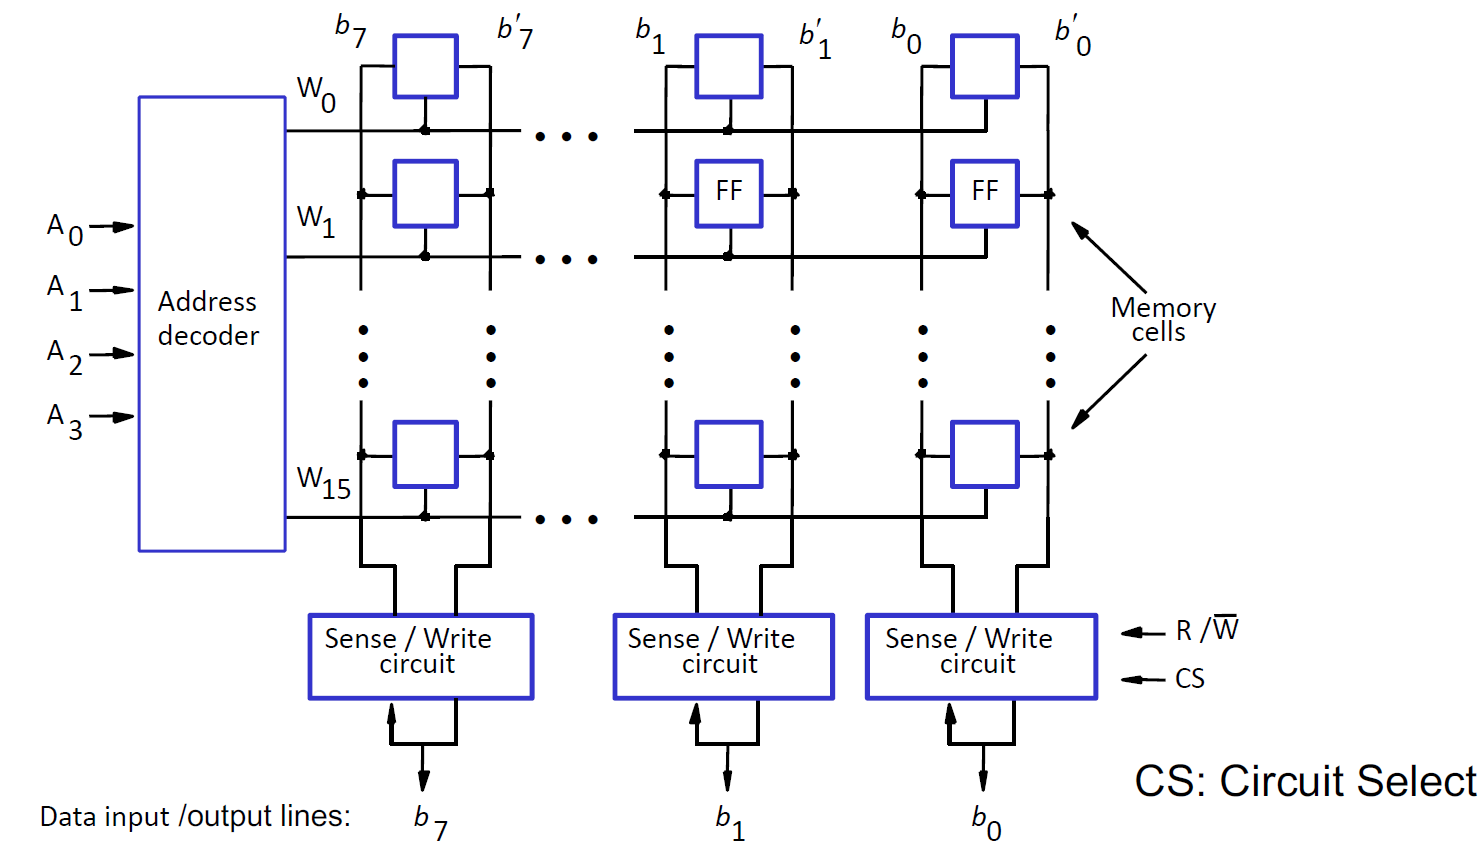
\includegraphics[width=\textwidth,keepaspectratio]{organizzazione.png}
	\caption{Organizzazione di un banco di memoria 16x8}
\end{figure}
Il caso presentato descrive il funzionamento di un banco di memoria formato da 16 righe e 8 colonne, con celle da un byte ciascuna. Si noti che per indirizzare un certo elemento all'interno della matrice del banco di memoria è necessario attivare una determinata riga e colonna (come avverrebbe in battaglia navale). Analizziamo ora, in ordine temporale, le operazioni che permettono di accedere/scrivere un determinato dato.
\begin{enumerate}
	\item In base alla riga da selezionare, l'\emph{address decoder} genera un 1 nell'uscita della riga corrispondente;
	\item Avviene un meccanismo simile anche per le colonne, attraverso il \emph{circuit select}, che decide se abilitare ciascuna colonna;
	\item Ogni colonna è gestita da un \emph{Sense/Write circuit} che riceve in input due linee di controllo: una definisce se eseguire l'operazione di lettura o scrittura (\emph{\(\textrm{R/}\overline{W}\)}) mentre l'altra (\emph{CS}) definisce se attivare o meno la colonna. Nel caso di una read, legge il valore contenuto nel bus della colonna (1 byte nel nostro esempio), altrimenti, nel caso di write, fa circolare il valore che si vuole scrivere nel bus della colonna. Per avere certezza dell'integrità dei dati viene propagato sia il dato stesso che si vuole scrivere che il suo negato. Ad esempio, nella colonna 0, \(b_0\) contiene il dato asserito, mentre \(b'_0\) contiene il dato negato;
	\item In base a com'è stata implementata la memoria (\emph{SRAM} o \emph{DRAM}), viene attivata la cella selezionata dalla colonna e dalla riga designata: su di essa verrà eseguita l'operazione di lettura/scrittura richiesta.
\end{enumerate}

Nelle prossime sezioni affronteremo le diverse implementazioni di cella di memoria: \emph{SRAM} e \emph{DRAM}.

\subsection{Le SRAM}
Le \emph{SRAM}, ossia le RAM statiche, sono delle memorie in cui i bit possono essere mantenuti indefinitivamente (posto il fatto che non manchi l'alimentazione). Seppur abbiano tempi di accesso molto ridotti (nell'ordine di pochi nanosecondi) e consumino poca corrente, il loro costo è molto elevato: per ciascuna cella di memorizzazione vengono impiegati molteplici componenti.
Il funzionamento che sta alla base di una cella di SRAM è quello del flip flop (in particolare ai latch tipo D).

\begin{figure}[H]
	\centering
	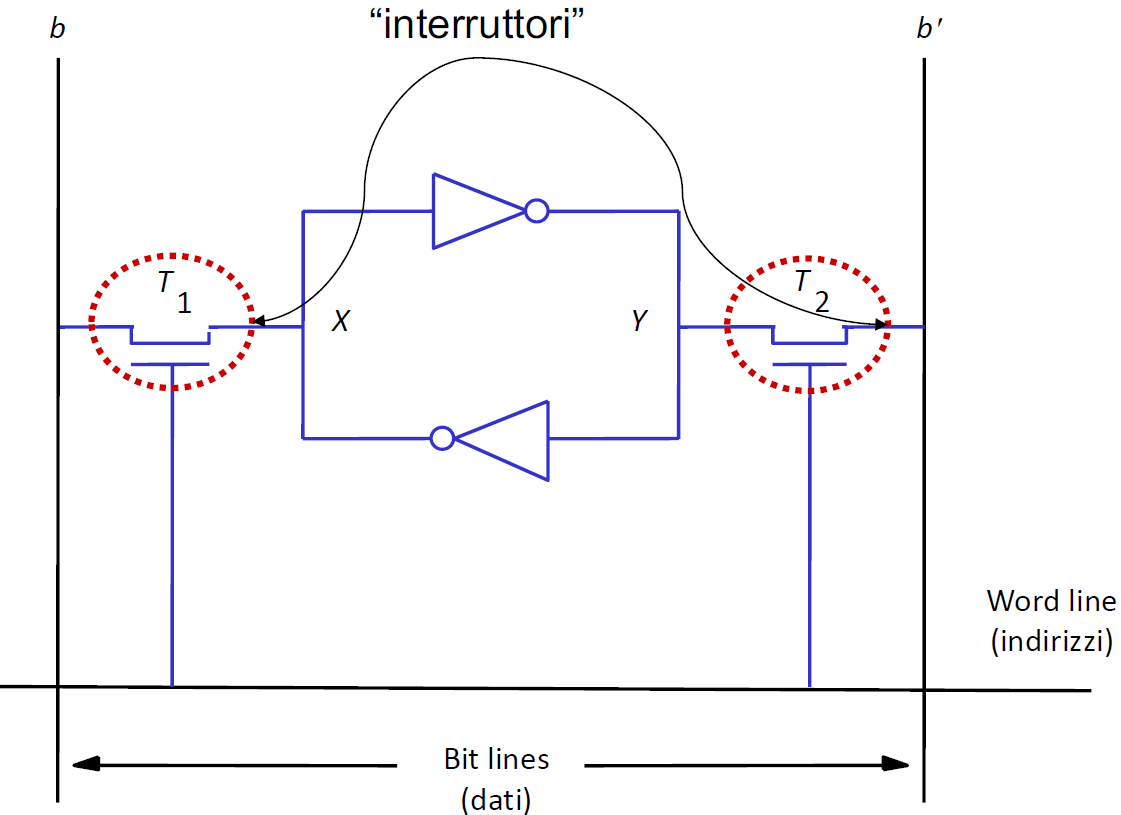
\includegraphics[width=0.7\textwidth,keepaspectratio]{cella_SRAM.png}
	\caption{SRAM: memorizzazione di un bit}
\end{figure}

Nell'immagine, \(\textrm{T}_1\) e \(\textrm{T}_2\) sono due transistor\footnote{Attraverso gli ultimi ritrovati dell'ingegneria, è possibile realizzare dei transistor nell'ordine di grandezza dei nanometri.}: in base al variare della tensione nel loro \emph{gate} (ossia il collegamento inferiore) permettono o meno il passaggio di corrente fra i rami laterali. Il funzionamento ricorda molto quello di un interruttore: se il gate ha ua tensione pari a Vdd, allora il circuito viene chiuso, altrimenti rimane aperto. Si noti che se la linea della word è bassa, allora gli interruttori \(\textrm{T}_1\) e \(\textrm{T}_2\) sono aperti e il consumo è praticamente nullo.

Dunque, nel caso venga chiuso il circuito, è possibile effettuare delle operazioni di lettura e di scrittura (gestite dal \emph{Sense/Write circuit}). Invece, nel caso in cui il circuito venisse aperto, la corrente circola solamente all'interno del latch a doppio NOT. La presenza di due NOT permette di rinforzare il risultato e ridurre il tasso di errore, in quanto si vuole controllare la coerenza delle informazioni sia col segnale \emph{b} che col segnale \emph{b'} (si ricorda che \emph{b} contiene il segnale asserito, mentre \emph{b'} contiene il segnale negato: \emph{b}\(=\)\emph{\(\overline{b'}\)}).

\subsection{Le DRAM}
Le \emph{DRAM}, ossia le RAM dinamiche, sono le memorie più diffuse nei computer. Sono dotate di costi molto contenuti e di un'elevatissima densità, dovuta al fatto di dover impiegare un solo componente per ogni singola cella di memoria. Il concetto che sta alla base della DRAM è un circuito RC (la resistenza è quella data dal filo): la capacità di memorizzazione viene ottenuta attraverso la carica di un condensatore. Presentano però un difetto che comporta consumi molto elevati: la cella di memoria necessita di un refresh continuo, altrimenti il proprio contenuto svanisce a causa delle correnti parassite e per la scarica del condensatore.

\begin{figure}[H]
	\centering
	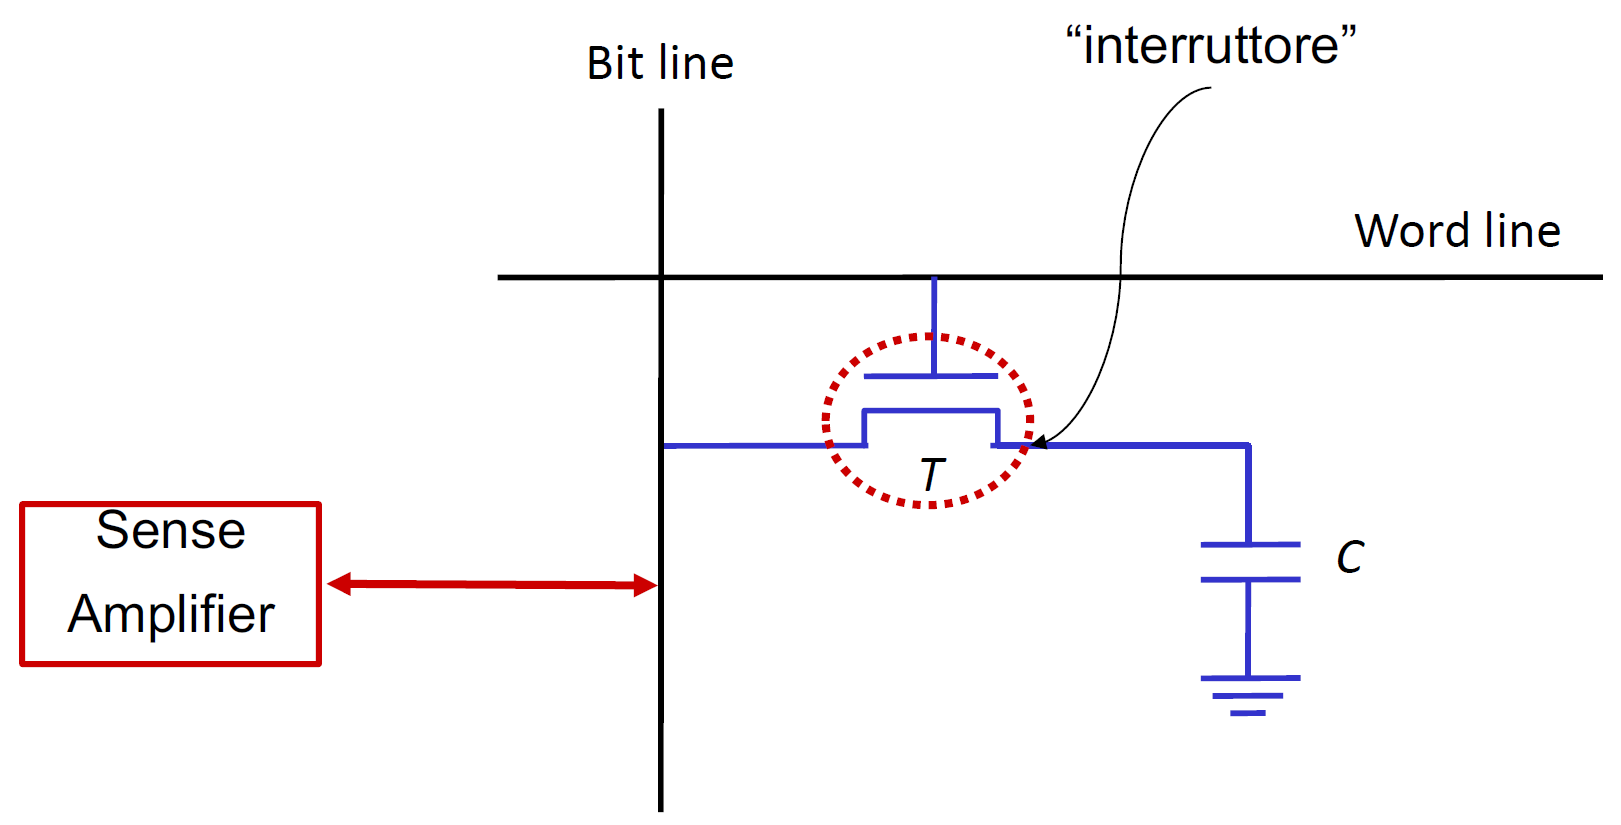
\includegraphics[width=0.7\textwidth,keepaspectratio]{cella_DRAM.png}
	\caption{DRAM: memorizzazione di un bit}
\end{figure}

Nell'immagine \(\textrm{T}\) è un transistor: svolge una funzione di interruttore, in quanto permette di collegare o meno il circuito RC alla bit line e alla word line. Se il circuito viene chiuso il condensatore viene caricato, altrimenti si scarica (ricordiamo che il processo di carica/scarica di un condensatore è esponenziale). Si ricorda che se non viene attivata la bit line o la word line, allora il circuito RC è scollegato, con la conseguente scarica del condensatore a causa della resistenza applicata. Dunque, se si vuole mantenere in memoria il dato 1, c'è la necessità di continuare a scrivere 1 nella cella di memoria ad ogni intervallo \(t_0\), altrimenti la scarica del condensatore annullerebbe il valore. Se il valore che si vuole memorizzare è 0, basta semplicemente lasciare disattivato il circuito (attenzione ad avergli lasciato il tempo necessario affinché si scarichi). Dunque per "refreshare" la memoria basta fare un ciclo di lettura: questo processo viene eseguito da un circuito di refresh, in maniera tale che l'utente non si debba preoccupare di questo meccanismo.\\
Si noti che nelle memorie DRAM non è implementato il latch a doppio NOT.\\
Solitamente si può considerare un condensatore scarico nel momento in cui la tensione ai suoi capi è inferiore a \(\frac{\textrm{Vdd}}{2}\). In particolare è proprio questo il compito del circuito \emph{sense amplifier}, il quale determina lo stato asserito o negato del dato memorizzato in base alla soglia \(\frac{\textrm{Vdd}}{2}\).

\subsubsection{La multiplazione degli indirizzi}
Facciamo un salto indietro di astrazione. L'immagine rappresenta l'organizzazione di una DRAM. \(A\) è l'indirizzo con cui si indicizza un dato in memoria: dalla posizione 20 a 9 definisce il valore da dare in input al decoder delle righe, dalla posizione 8 alla 0 definisce il valore da dare al decoder delle colonne. Questa DRAM è caratterizzata da 4096 (\(2^{12}\), dove 12 rappresenta il numeri di bit di A per indirizzare la riga) righe e 512 (\(2^9\), dove 9 rappresenta il numero di bit di A per indirizzare la colonna) colonne:
\begin{figure}[H]
	\centering
	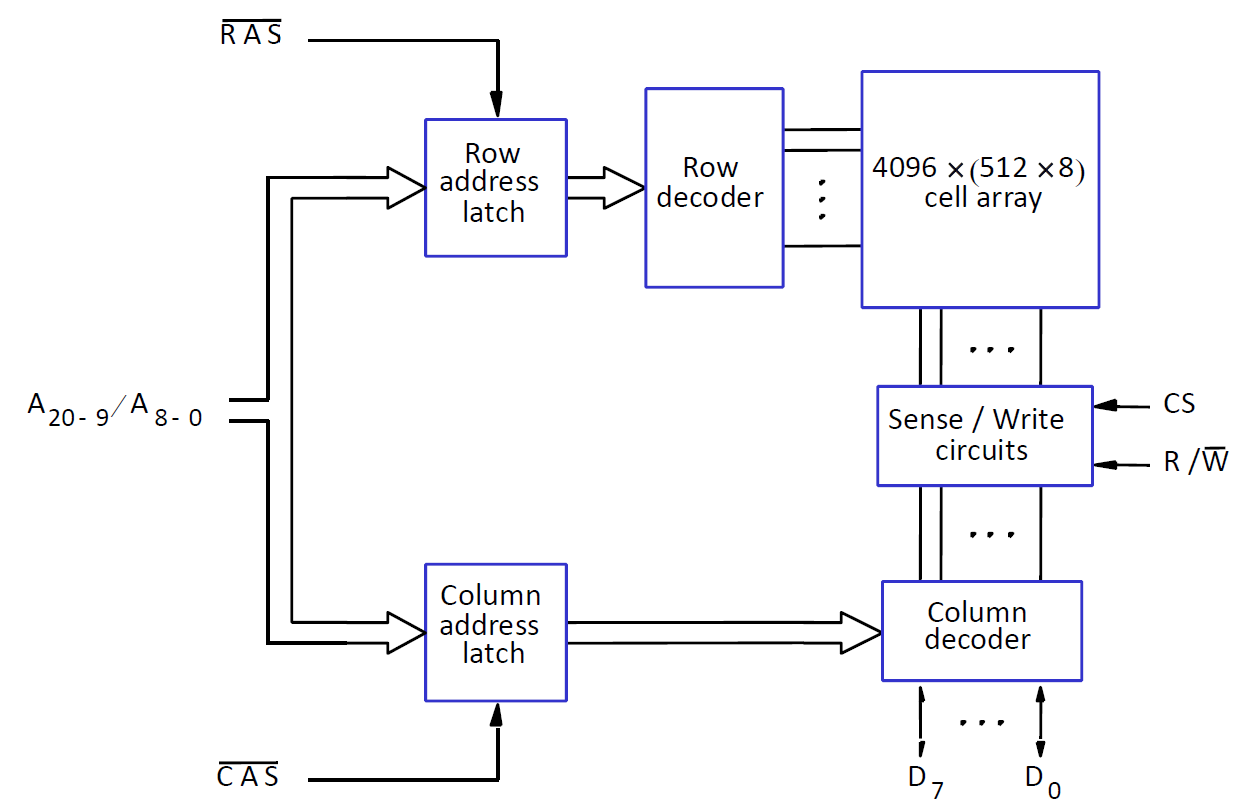
\includegraphics[width=0.7\textwidth,keepaspectratio]{organizzazione_generale.png}
	\caption{Organizzazione generale di una memoria}
\end{figure}
Si noti che sono stati inseriti due circuiti: \emph{row address latch} e \emph{column address latch}, che rispettivamente ricevono in input i codici di controllo \emph{\(\overline{RAS}\)} e \emph{\(\overline{CAS}\)}. Queste due linee di controllo permettono di decidere, in base al loro input, se è possibile accedere ad una riga/colonna.

\subsubsection{Fast Page Mode (FPM)}\label{sec:FPM}
Solitamente i trasferimenti da/per la memoria avvengono a blocchi piuttosto che per singole celle. Ciò comporta un notevole risparmio di tempo, in quanto sarebbe necessario solo un unico indirizzamento per le righe e colonne. Questo processo viene chiamato \emph{fast page mode} (\emph{FPM}). Si sottolinea che questa modalità è del tutto automatica: l'utente non deve preoccuparsi di gestire questo meccanismo.

\subsubsection{Le DRAM sincrone}
Le DRAM che sono state descritte fin'ora sono dette \emph{asincrone}, in quanto non esiste una precisa temporizzazione di accesso: la dinamica viene governata dai segnali \emph{\(\overline{RAS}\)} e \emph{\(\overline{CAS}\)}. Si noti che questa asincronicità può causare non pochi problemi, soprattutto mentre si esegue il refresh della memoria. Una soluzione consiste nell'aggiungere dei buffer di memorizzazione degli ingressi e delle uscite, in maniera tale da riuscire a disaccoppiare la lettura e scrittura dal refresh della memoria, ottenendo automaticamente un accesso FPM pilotato dal clock. Questa implementazione della DRAM viene detta \emph{sincrona}. A seguire un'immagine che contiene uno schema riassuntivo:
\begin{figure}[H]
	\centering
	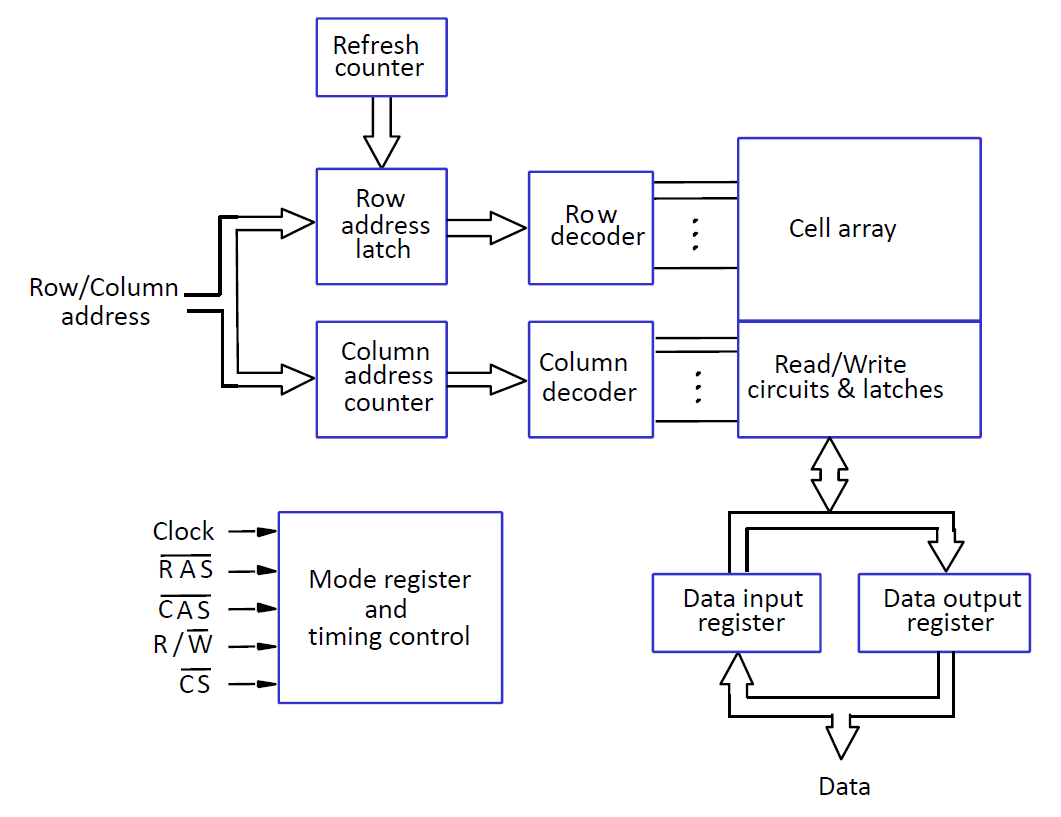
\includegraphics[width=0.9\textwidth,keepaspectratio]{DRAM_sincrona.png}
	\caption{Organizzazione generale di una DRAM sincrona}
\end{figure}

Nella prossima immagine è possibile visualizzare un accesso sincrono in FPM:
\begin{figure}[H]
	\centering
	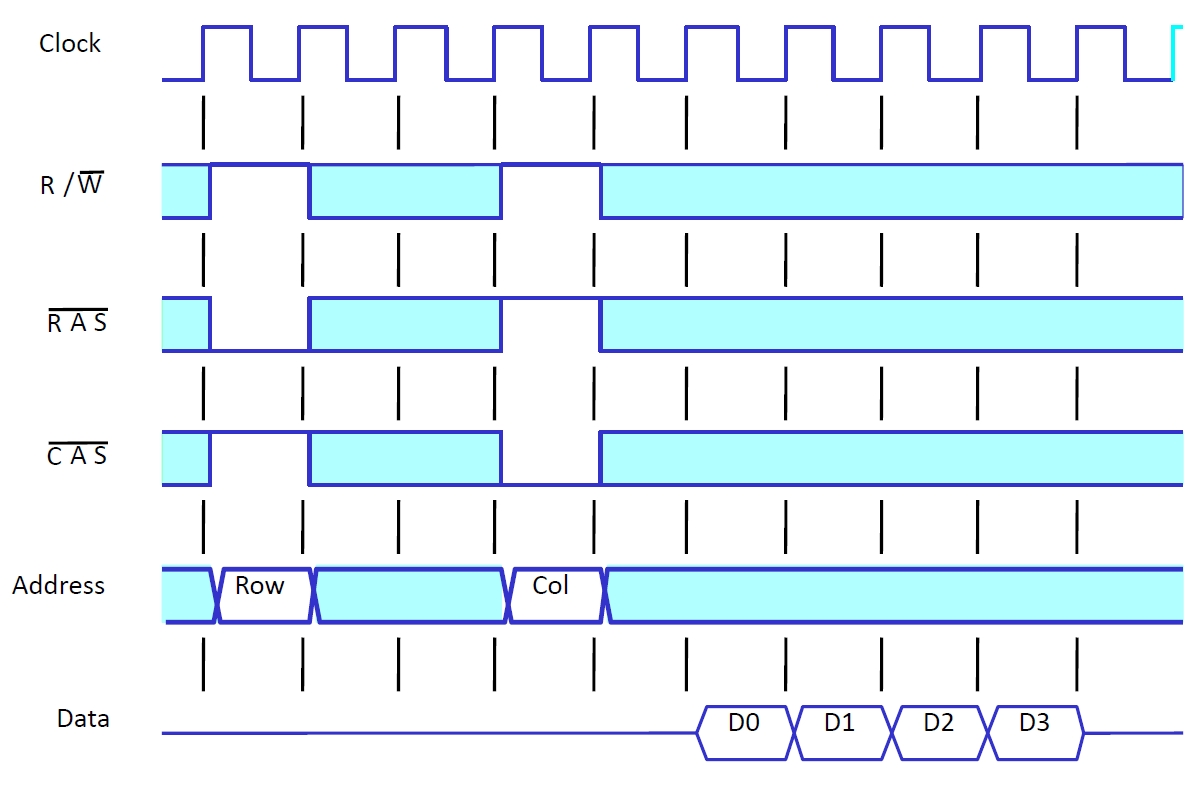
\includegraphics[width=0.7\textwidth,keepaspectratio]{FPM.png}
	\caption{Funzionamento fast page mode}
\end{figure}
dove il segnale di clock rappresentato è quello della memoria RAM: le operazioni di lettura e scrittura sono sincronizzate col fronte di salita; D0, D1, D2, D3 sono i byte che arrivano in serie; i valori rimanenti sono le linee di controllo.

\subsubsection{Double Data Rate SDRAM (DDR-SDRAM)}
Un ulteriore miglioramento è effettuato dalla \emph{DDR-SDRAM} (\emph{Double Data Rate SDRAM}): essa permette il trasferimento dei dati sia sul fronte di salita che sul fronte di discesa del clock della memoria. In poche parole ciò permette di raddoppiare le prestazioni rispetto ad una normale SDRAM, e nonostante la latenza rimanga invariata, la banda viene raddoppiata.

Sono ottenute organizzando la memoria in due banchi separati: uno contiene le posizioni pari (a cui si accede durante il fronte di salita), l'altro contiene quelle dispari (a cui si accede durante il fronte di discesa). Locazioni contingue risultano divise fra i due banchi: grazie a questo è possibile effettuare un accesso in modo interlacciato.

\section{Gestione della memoria}
Andiamo adesso a domandarci quale possa essere il modo migliore di gestire la memoria che abbiamo a disposizione. È preferibile conservare i dati nella memoria RAM? Così facendo possiamo avere dei tempi di accesso ai dati estremamente ridotti, ma di contro la quantità di dati di cui possiamo disporre sarà limitata. Dobbiamo quindi affidare i nostri dati alle memorie periferiche? In questo modo possiamo avere moltissimo spazio dove riporre i nostri dati, ma il tempo necessario a raggiungere di volta in volta quelli che ci servono sarà decisamente maggiore.

L'approccio vincente è quello di mantenere i dati archiviati nelle memorie periferiche (dove lo spazio abbonda), e ogniqualvolta siano necessari prelevarli e caricarli sulla RAM; quando questa sarà piena, i dati non più necessari verranno riarchiviati per far spazio a quelli nuovi. In questo modo possiamo avere botte piena e moglie ubriaca, perché possediamo una grande quantità di dati archiviati e possiamo accedere alla maggior parte di questi in modo veloce. Andiamo a formalizzare quanto appena detto nei due seguenti \emph{principî di località}.
\begin{itemize}
	\item \emph{Principio di località temporale}: questo principio dice che se faccio uso di un dato in memoria è molto probabile che nel breve periodo dovrò servirmene di nuovo. Ad esempio, se ci troviamo all'interno di un ciclo, dovrò accedere alle stesse zone di memoria ad ogni iterazione.
	\item \emph{Principio di località spaziale}: questo principio dice invece che quando accedo a una locazione di memoria è molto probabile che io debba accedere anche a zone a lei adiacenti (o contigue); questo per esempio succede ogni volta che dobbiamo lavorare per gli array, che sono ordinati per word successive.
\end{itemize}

\subsection{Struttura della gerarchia}
Osserviamo la seguente tabella:
\begin{figure}[H]
	\centering
	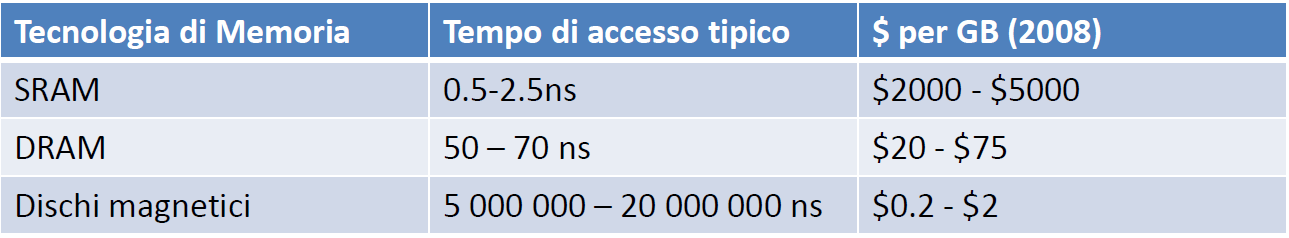
\includegraphics[width=\textwidth,keepaspectratio]{tabella_polli.png}
\end{figure}
Al di là dei dati un po' desueti\footnote{Verrebbe quasi da dire che fanno ridere i polli, in effetti.}, si può facilmente intuire quale sarà la gerarchia delle memorie: quelle più veloci ma costose saranno vicine al processore e gli forniranno i dati da elaborare, mentre invece quelle più lente (ma più capienti) staranno lontane e fungeranno da archivio.
\begin{figure}[H]
	\centering
	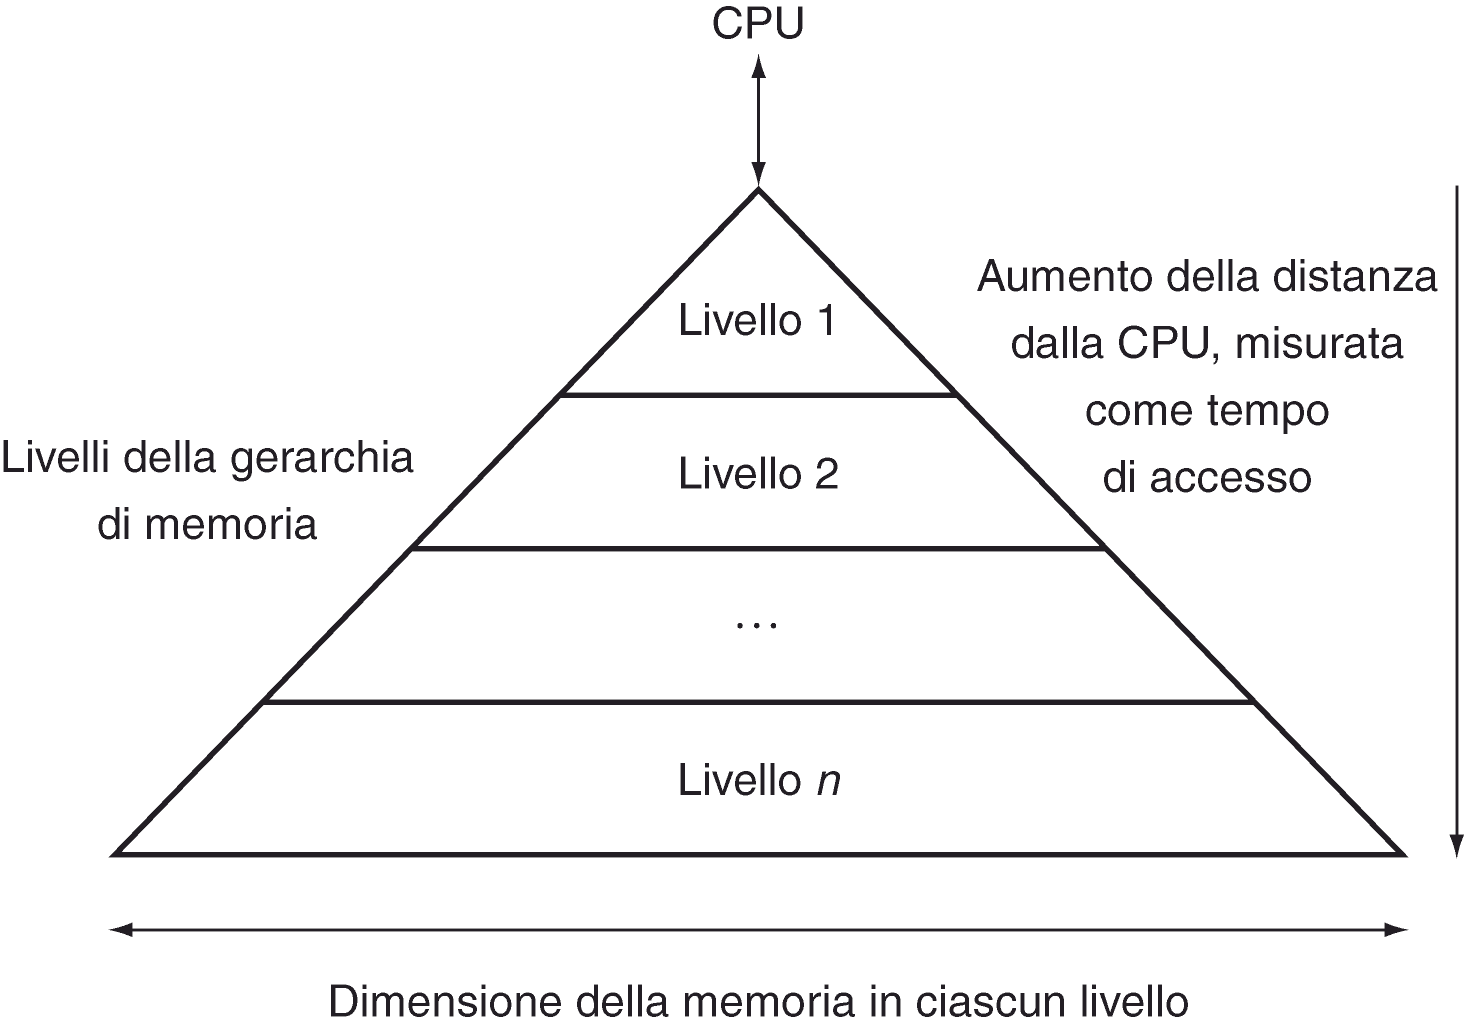
\includegraphics[width=0.6\textwidth,keepaspectratio]{strut-ger.png}
	\caption{Struttura gerarchica delle memorie}
\end{figure}

\section{La cache}
La cache (dal francese \emph{caché}, participio passato del verbo \emph{cacehr}, "nascondere") è una memoria molto vicina al processore e invisibile al programmatore; dopo essere stata sperimentata negli anni '70 è diventata parte della progettazione di ogni tipo di calcolatore.

\subsection*{Altre definizioni}
Forniamo ora una breve carrellata di definizioni cui bisogna prendere familiarità per affrontare la seguente sezione.
\begin{itemize}
	\item \emph{Blocco}: unità minima dell'informazione che può essere presente o assente in un livello superiore a quello di riferimento.
	\item \emph{Hit rate}: frequenza di successo, ossia il rapporto tra il numero di accessi al livello superiore in cui trovo il dato e il numero totale di accessi che compio.
	\item \emph{Miss rate}: \(1 - \textrm{\emph{hit rate}}\), frequenza degli insuccessi.
	\item \emph{Hit time}: tempo che occorre a leggere il dato una volta individuato il blocco al livello superiore.
	\item \emph{Miss penalty}: tempo che occorre ad accedere al dato se non trovo il blocco al livello superiore.
\end{itemize}

\subsection{Cache a mappatura diretta}\label{sec:direttamente}
Ma come si può sapere se un determinato dato è nella cache? Com'è è possibile eventualmente cercarlo?

Un sistema interessante per gestire la cache potrebbe essere quello detto \emph{a mappatura diretta}: ad ogni indirizzo in memoria corrisponde una precisa locazione di cache; l'indirizzo in cache viene normalmente mappato come segue:

\begin{equation*}
	\textrm{indirizzo in cache} \equiv \textrm{indirizzo in memoria}  \pmod{\textrm{numero blocchi cache}}
\end{equation*}

Qualora il numero di blocchi in cache fosse potenza di due sarà sufficiente usare i bit meno significativi del loro indirizzo in memoria. Quanti bit meno significativi bisogna prendere, di preciso? La risposta è in questa formula:
\begin{equation*}
	\textrm{Cache address}=\log_2 (\textrm{cache dimension})
\end{equation*}
Se per esempio abbiamo una cache di 8 parole dobbiamo prendere i 3 bit meno significativi dell'indirizzo in memoria, come illustrato dalla seguente immagine.
Si noti che l'operazione di modulo e di logaritmo restituiscono lo stesso risultato, sono perfettamente equivalenti.
\begin{figure}[H]
	\centering
	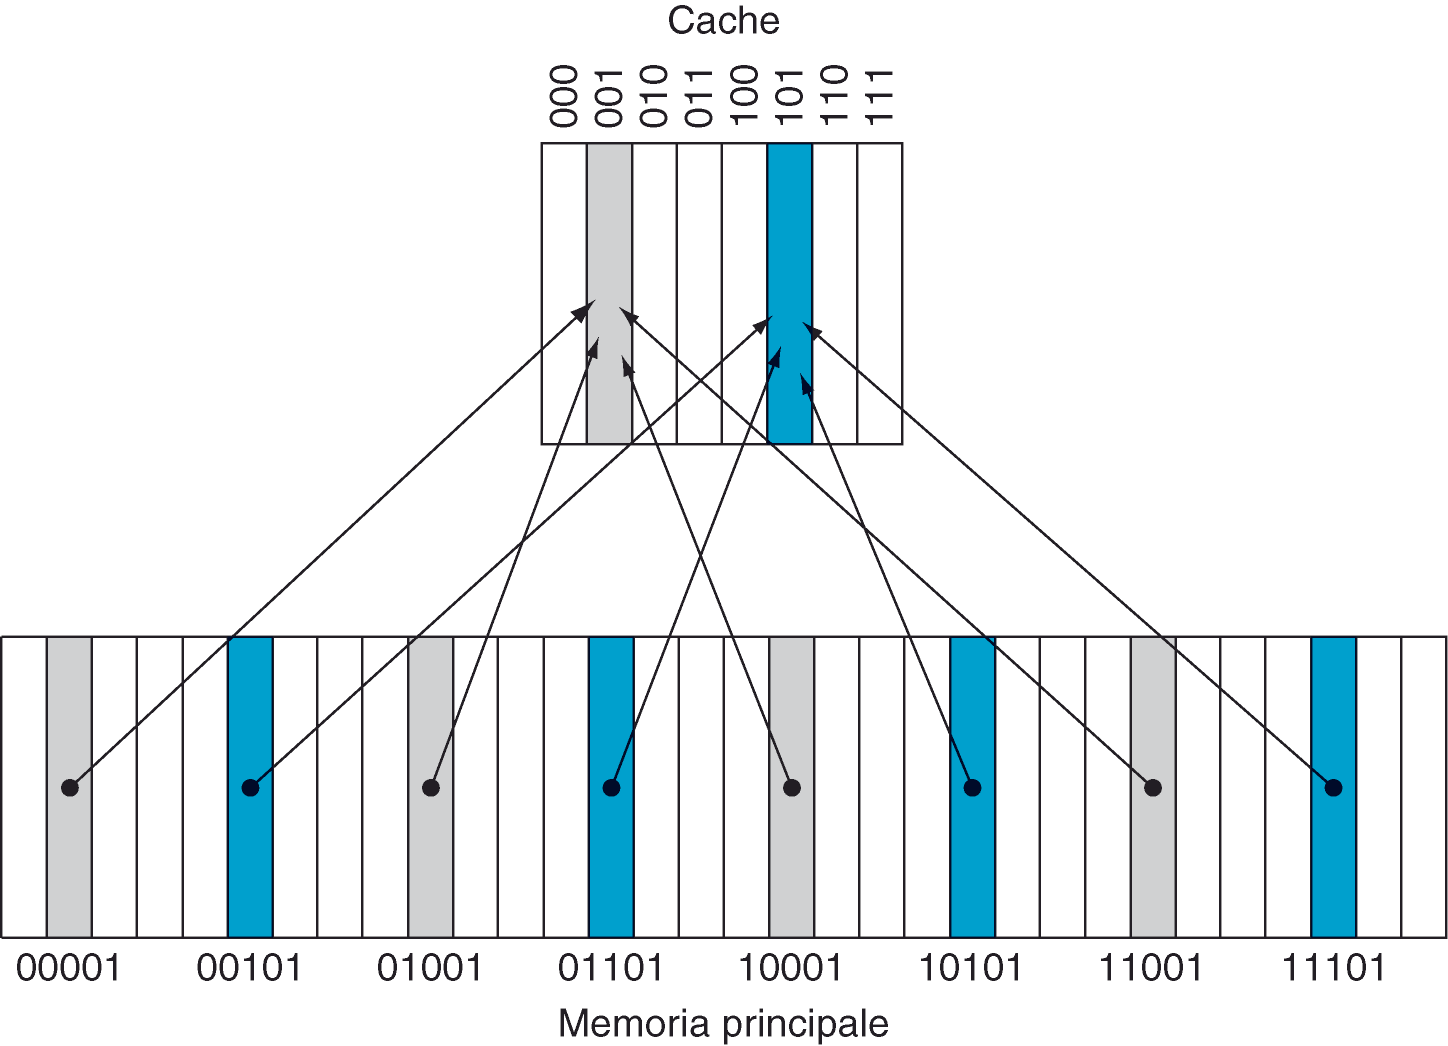
\includegraphics[width=0.8\textwidth,keepaspectratio]{logad.png}
	\caption{Esempio di mappatura da memoria a cache}
\end{figure}
Dal momento che molte parole in memoria possono ritrovarsi mappate nel medesimo blocco di cache sarà necessario ricorrere a dei \emph{tag} identificativi; i bit non utilizzati per l'indirizzamento adempiscono egregiamente allo scopo. L'ultimo elemento che vediamo è un cosiddetto \emph{bit di validità}, fornito dal gestore della cache (quindi non prelevato dall'indirizzo del blocco) che ci dice se quello che in un dato momento abbiamo memorizzato in un blocco di cache sia valido o meno.

\subsection{La cache in MIPS}
Adesso mostriamo un esempio di come viene gestita la cache in Assembly MIPS. Assumiamo le seguenti informazioni:
\begin{itemize}
	\item gli indirizzi sono vettori di 32 bit, naturalmente;
	\item la cache seguirà il criterio della mappatura diretta prima descritto;
	\item la cache avrà dimensione \(2^{n}\) blocchi, di cui \(n\) bit usati per l'indice di ogni blocco;
	\item il blocco di cache sarà composto di \(2^{m}\) parole, ossia \(2^{m+2}\) bit\footnote{La ragione di quel \(m + 2\) è naturalmente nel fatto che le parole sono sempre linee di 4 bytes, per cui il loro numero va sempre moltiplicato per \(4\), ossia \(2^{2}\); vediamo i \(2\) bit riservati a questo offset anche nell'immagine sottostante.};
	\item la dimensione del \emph{tag} sarà di \(32-(n+m+2)\) bit.
\end{itemize}
Si analizzi attentamente la seguente immagine, tenendo presente che \(n=10\) e \(m=0\), quindi la dimensione del \emph{tag} è di \(20\) bit.

\begin{figure}[H]
	\centering
	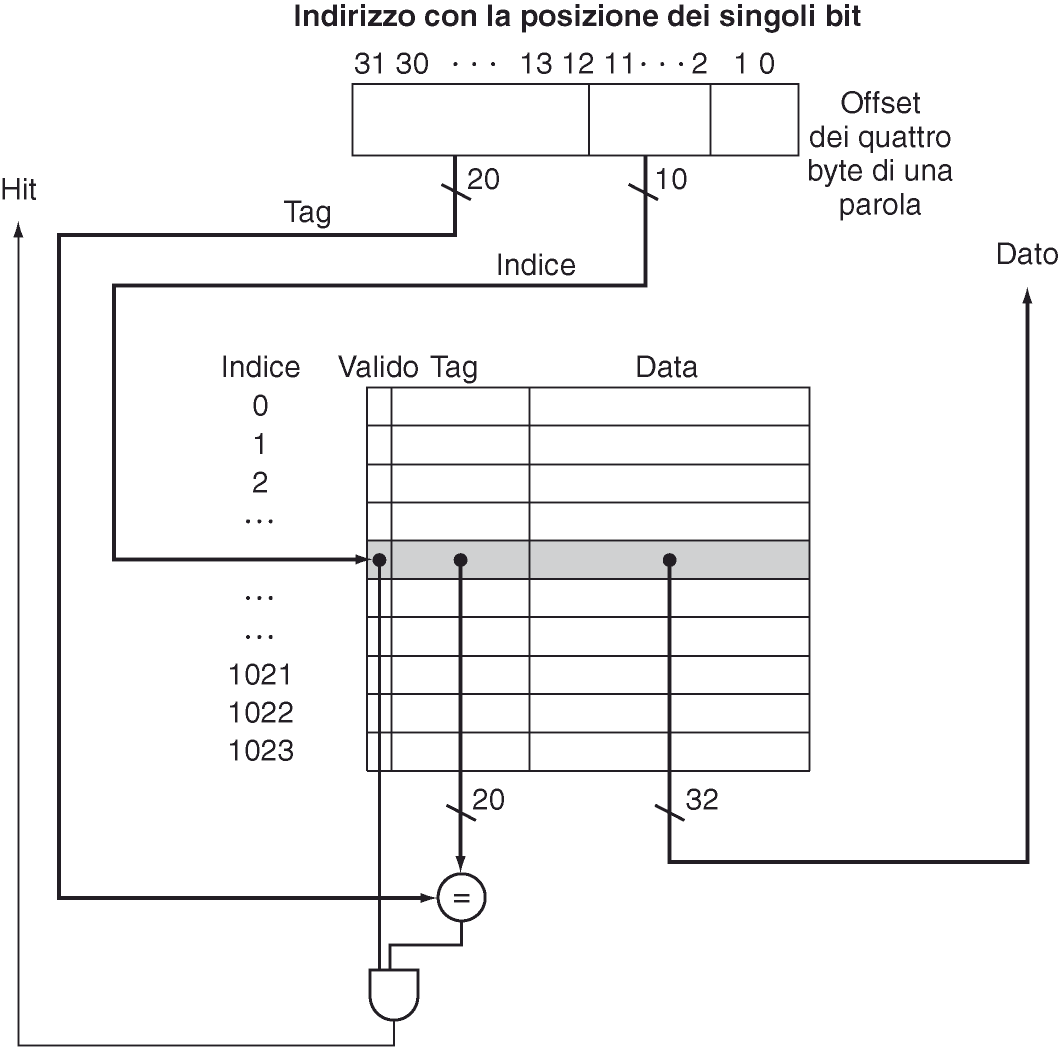
\includegraphics[width=0.7\textwidth,keepaspectratio]{mipscache.png}
	\caption{Schema risoluzione indirizzo}
\end{figure}

\subsubsection{Il calcolo degli indirizzi}
Mostriamo con un esempio come calcolare a quale blocco di cache corrisponde un determinato indirizzo in memoria.

Supponiamo di avere una cache con \(64\) blocchi di \(16\) byte ciascuno e di voler trovare a quale blocco cache corrisponde l'indirizzo 1200 in byte. Ricordiamo che l'indirizzo di ogni blocco è identificato da:
\begin{equation*}
	\textrm{Indirizzo blocco}\pmod{\textrm{Numero di blocchi della cache}}
\end{equation*}
con l'indirizzo del blocco definito come segue:
\begin{equation*}
	\textrm{Indirizzo blocco}=\frac{\textrm{Indirizzo dato in byte}}{\textrm{Byte per blocco}}
\end{equation*}
\begin{itemize}
	\item Calcoliamo l'indirizzo del blocco: \(\frac{1200}{16}=75\)
	\item A questo punto calcoliamo l'indirizzo del blocco nella cache corrispondente: \(75\pmod{64}=11\)
\end{itemize}
Il blocco di cache cercato è quindi il numero \(11\).

\begin{figure}[H]
	\centering
	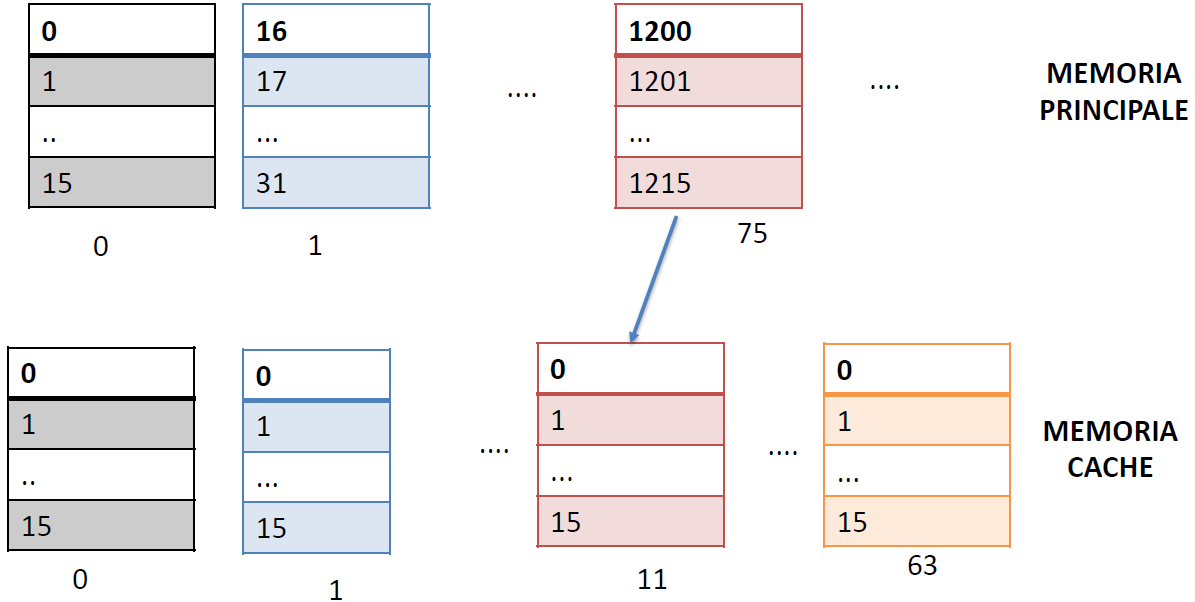
\includegraphics[width=0.8\textwidth,keepaspectratio]{addressex.png}
	\caption{Esempio di calcolo blocco}
\end{figure}

\subsection{La ricerca di un compromesso}
A questo punto risulta evidente che avere blocchi di cache molto grandi ci permette di sfruttare ampiamente il principio della località spaziale, dal momento che disporrò di molto spazio in cui riporre gruppi di dati anche di dimensioni importanti; perché non si ricorre sempre a una soluzione di questo tipo, allora? Perché innanzitutto avere blocchi molto grandi porta a dei costi di gestione molto alti (di fatto di volta in volta ci troviamo a spostare molti byte), ma soprattutto perché a parità di dimensioni avere meno blocchi diminuisce l'efficacia della località temporale. Per questo motivo è molto importante trovare un buon compromesso tra numero di blocchi e dimensione degli stessi, in fase di progettazione.

La figura sottostante mostra come varia la frequenza delle miss (asse \(y\)) in relazione a diverse dimensioni di cache (le varie linee) e in numeri di blocchi (asse \(x\)). Osserviamo che le migliori prestazioni le abbiamo sempre per valori equilibrati, e che la maggior differenza la osserviamo per dimensioni di cache più piccole.
\begin{figure}[H]
	\centering
	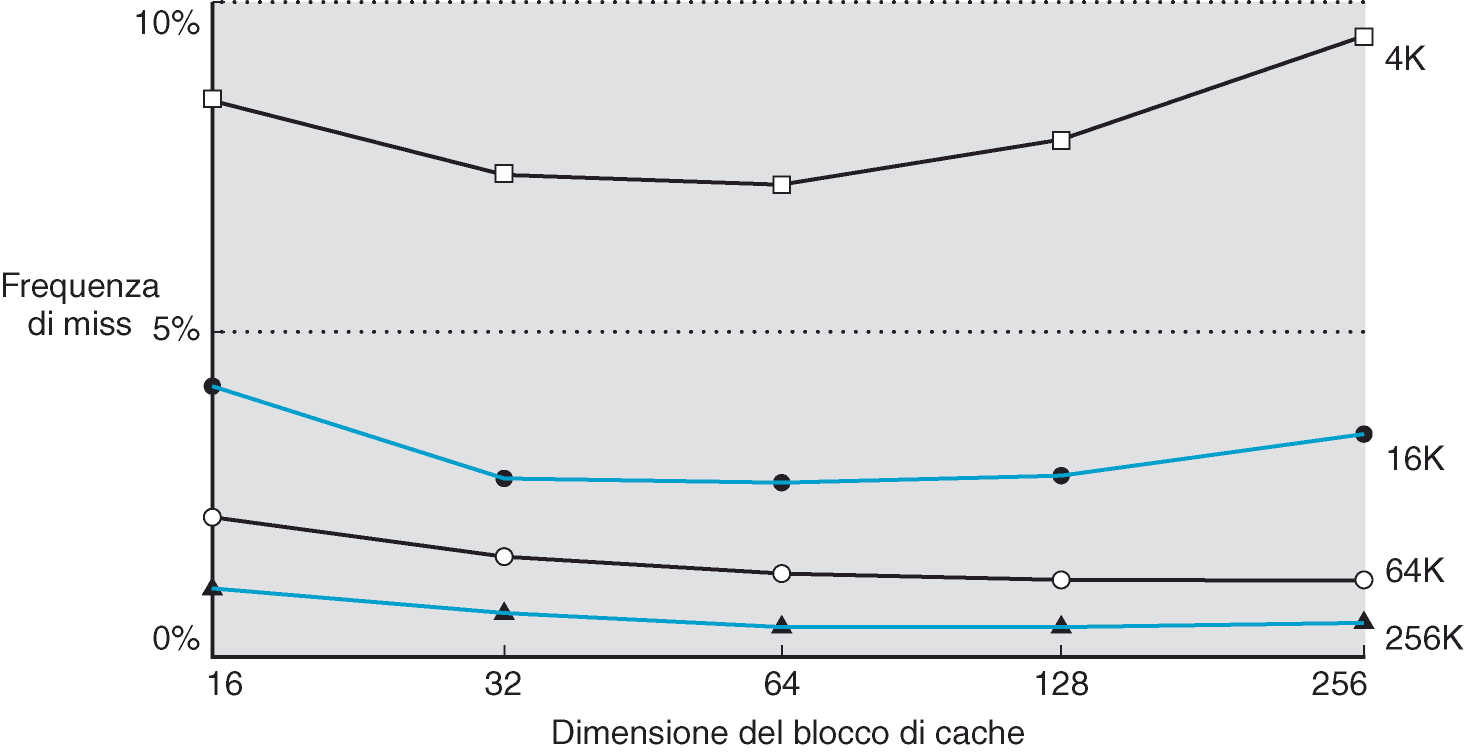
\includegraphics[width=0.8\textwidth,keepaspectratio]{missfreq.png}
\end{figure}

\subsection{Gestione delle miss}
Fintantoché non avviene una miss il funzionamento di una CPU con pipeline non viene influenzato dalla presenza della cache, ma quando una di queste viene riscontrata è necessario bloccare temporaneamente il flusso della pipeline e gestire il trasferimento dei dati dalla memoria principale alla cache. Vediamo come viene gestita una miss sulla memoria istruzioni.
\begin{enumerate}
	\item Inizialmente bisogna raddrizzare il program counter; ricordiamo che questo viene incrementato di \(4\) all'inizio di ogni istruzione, quindi l'eventuale miss sarà su \(PC-4\), e questo sarà infatti il valore che dobbiamo inviare alla memoria.
	\item Dobbiamo inviare alla memoria il comando di eseguire una lettura ed attenderne il completamento.
	\item A questo punto dobbiamo scrivere il dato proveniente dalla memoria in cache e aggiornarne i tag.
	\item Infine possiamo rieseguire il fetch e trovare adesso l'istruzione in cache al posto giusto.
\end{enumerate}

\subsection{Scritture}
Se gli accessi in lettura avvengono con la logica precedente, quelli in scrittura sono più delicati e potrebbero causare problemi di consistenza, ossia potrei avere situazioni in cui si genera un disallineamento tra i dati presenti in cache e quelli presenti nella memoria principale.
\begin{itemize}
	\item Un sistema che possiamo adoperare per arginare questo problema è il cosiddetto \emph{write-through}, che consiste nel fatto che ogni scrittura viene effettuata direttamente in memoria principale, a prescindere dal fatto che ci sia o meno una miss. In questo modo avrò cache e memoria sempre aggiornati, ma ben si capisce che si tratta di un'operazione costosa; una buona aggiunta potrebbe essere un buffer di scrittura, una sorta di "coda" dove tutte le scritture vengono messe in attesa, che ci permette quindi di accorpare il maggior numero di operazioni possibile e mantenere cache e memoria sempre allineate.
	\item Una seconda soluzione potrebbe essere la cosiddetta \emph{write-back}: se il blocco richiesto è già presente in cache allora ogni scrittura verrà fatta solo localmente e la memoria principale viene aggiornata solo quando si cambia il blocco di riferimento (oppure quando un secondo processore tenta di accedere allo stesso blocco); chiaramente questa soluzione è pensata in situazioni molto affollate, quanto il processore non riesce a processare in modo efficiente le molte scritture richieste.
\end{itemize}
Riportiamo come esempio \emph{FastMath}, una cache basata su MIPS che dispone di una cache di \(16K\) con \(16\) parole per blocco e la possibilità di lavorare sia in \emph{write-through} che in \emph{write-back}.

\begin{figure}[H]
	\centering
	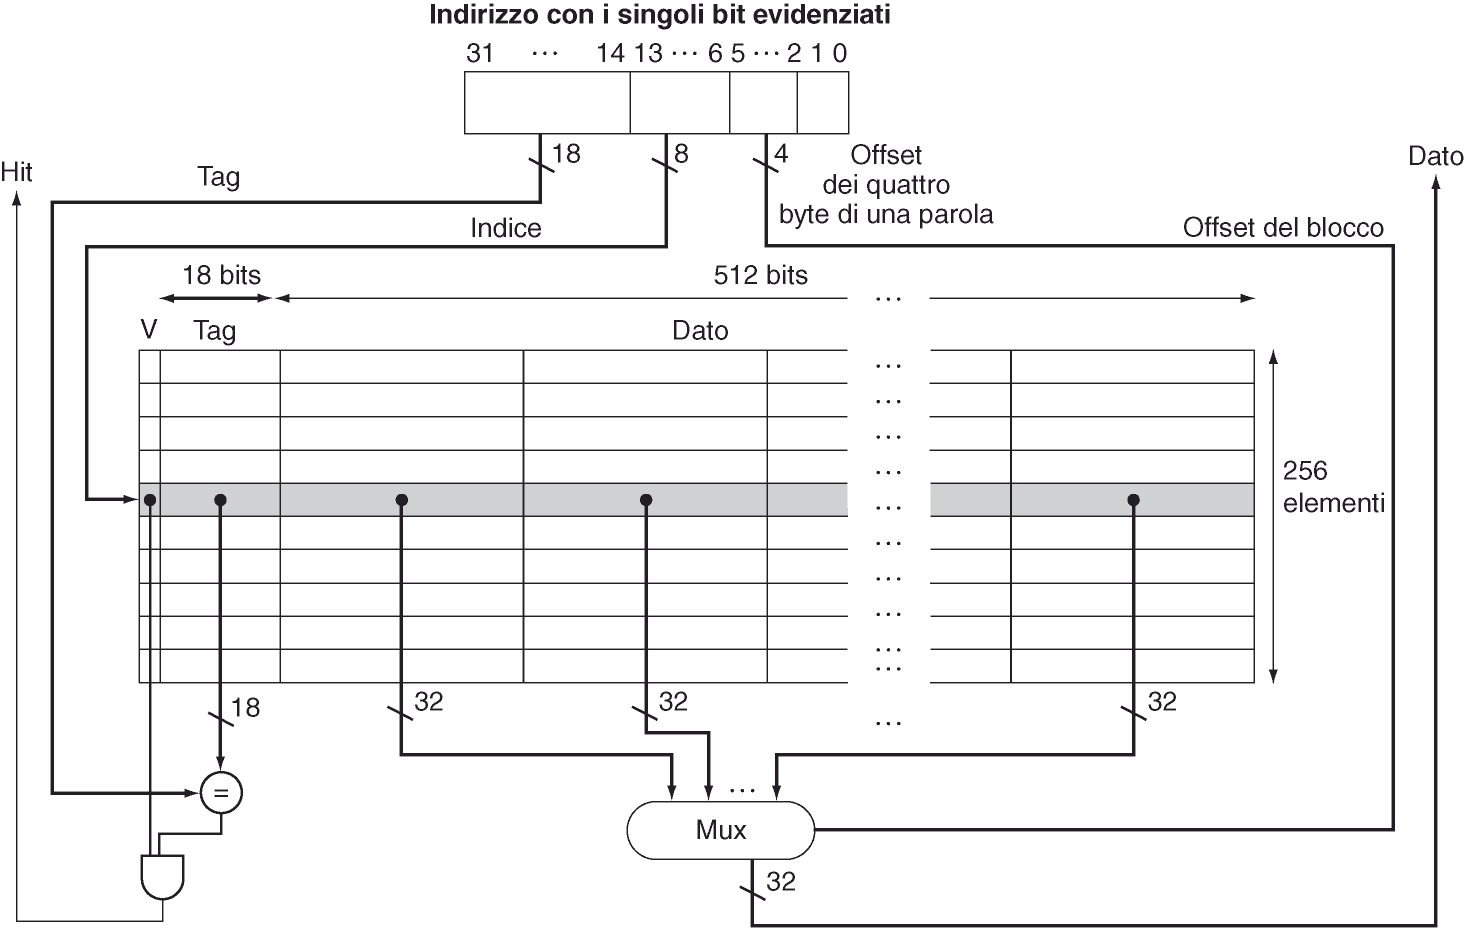
\includegraphics[width=0.9\textwidth,keepaspectratio]{astmips}
\end{figure}

\begin{itemize}
	\item Notiamo in basso a sinistra una porta AND: questa prenderà in input il bit di validità e il risultato del confronto tra il tag del blocco selezionato e l'indirizzo. Il risultato in output determinerà se avremo conseguito una \emph{hit} oppure no.
	\item Infine osserviamo un multiplexer in cui confluiscono tutte le \(16\) parole del blocco; per determinare quale word debba andare in output viene impiegato come segnale di controllo un offset dall'indirizzo del blocco di cache.
\end{itemize}

\section{Cache associative}
Le cache a mappatura diretta sono piuttosto semplici da realizzare, tuttavia presentano un problema: se ho spesso bisogno di locazioni di memoria che si mappano sullo stesso blocco di cache\footnote{Ricordiamo che questo significa che tali blocchi sono congrui in modulo \(n\).}, ho cache miss in continuazione.
Proprio per gestire queste situazioni è nata l'implementazione della cache completamente associativa.

\subsection{Cache completamente associativa}
Una cache completamente associativa è una cache in cui ogni blocco della memoria può essere mappato in un qualsiasi blocco della cache. Il problema in cui si incorre utilizzando cache completamente associative è che si deve cercare in tutta la cache il dato (il tag in questo tipo di cache è rappresentato da tutto l’indirizzo del blocco). Per effettuare la ricerca in maniera efficiente si deve quindi lanciarla su tutti i blocchi in parallelo.

Per questo motivo ho bisogno di $n$ comparatori (uno per ogni blocco di cache) che operino in parallelo; di conseguenza la complessità di realizzazione cresce proporzionalmente al numero di blocchi ed inoltre il costo HW diventa proibitivo appena si aumenta di poco la dimensione della memoria.

\subsection{Cache set-associativa}
Le cache set-associative sono una via di mezzo tra le due che abbiamo visto finora.
In una cache set-associativa, composta da $n$ blocchi totali, tutti i blocchi vengono suddivisi in un determinato numero di gruppi, che vengono chiamati linee; ogni gruppo di conseguenza contiene un numero pari a \(\frac{n}{\textrm{numero di linee}}\) di blocchi, che chiameremo vie.

Fatta questa suddivisione quello che si ottiene è una sorta di scacchiera in cui i blocchi possono essere visti in raggruppamenti di "linee" (righe) e di "vie" (colonne).

Riusciamo quindi ad ottenere una combinazione delle due diverse cache: mappiamo ciascun blocco della memoria centrale in una certa linea direttamente (vedi ~\ref{sec:direttamente}), in seguito questo può essere inserito in una qualsiasi delle vie in maniera associativa.

% un giorno potrebbe servire
%Ribadiamo per chiarezza che la cache set-associativa %lavora a mappatura diretta sulle linee ed in maniera %completamente associativa sulle vie (all'interno di una %stessa linea).

Quando si va a cercare un blocco quindi se ne calcola la linea in cui è mappato direttamente ed in seguito, all'interno di questa linea, si effettua una ricerca parallela su tutte le vie (come nelle cache completamente associative).

Il grande vantaggio è che abbiamo una memoria non troppo costosa, dato che la cache associativa viene implementata su blocchi di dimensioni ridotte; tuttavia si mantiene anche (almeno parzialmente) il vantaggio della strategia associativa con conseguente abbassamento del \emph{miss rate}.

È ora riportato uno schema con una cache suddivisa in più modi differenti, ma sempre attraverso la strategia di cache set-associativa, come esempio esplicativo; si noti che ogni gruppo Tag-Dato rappresenta una via.

\begin{figure}[H]
	\centering
	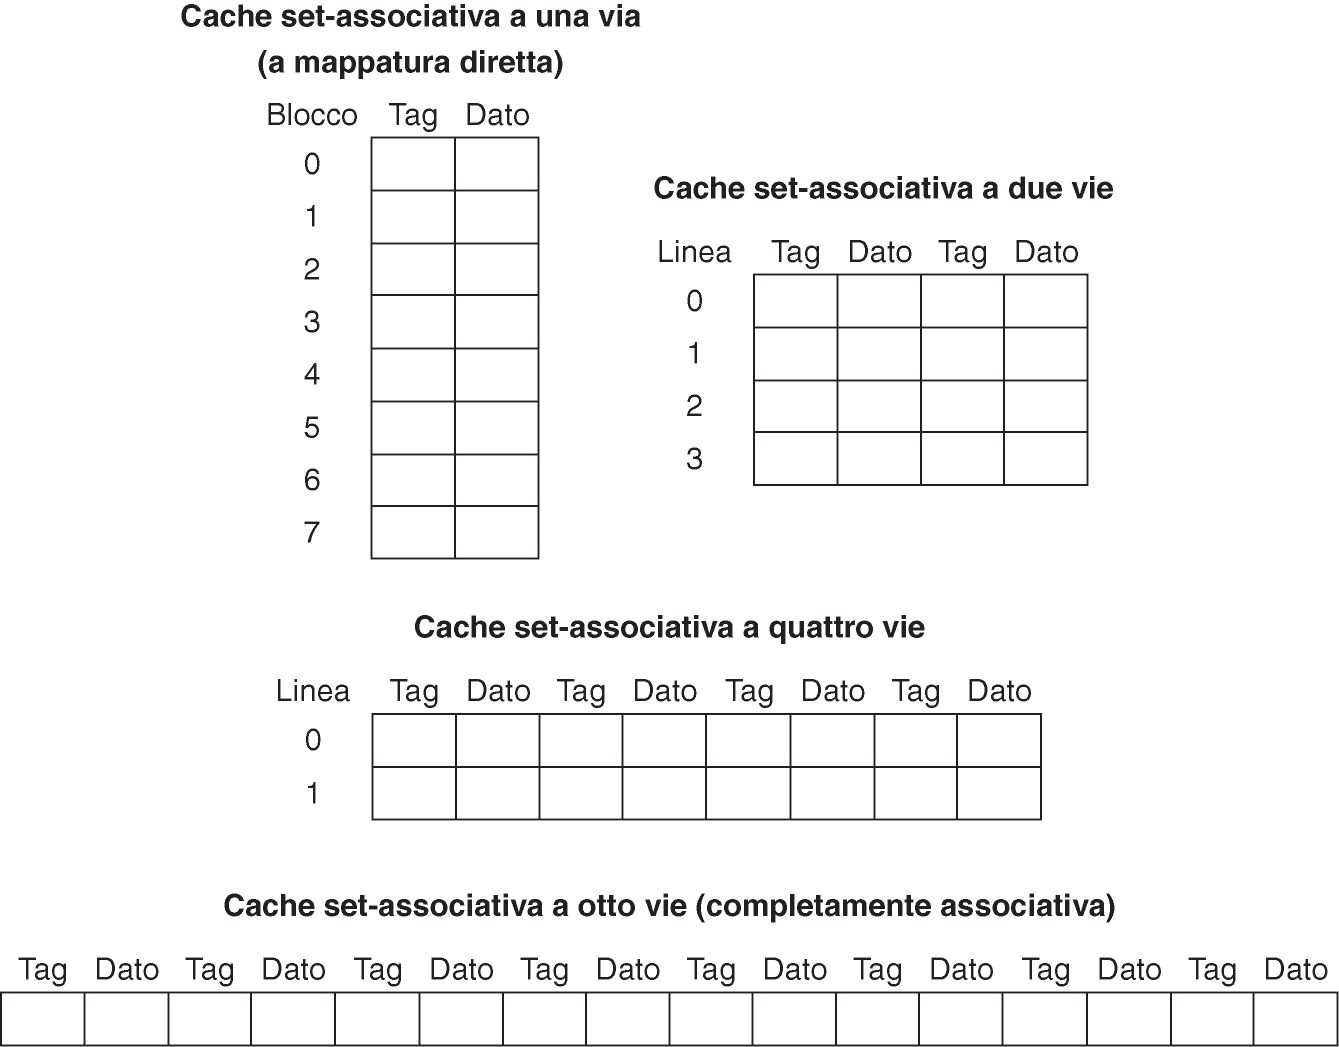
\includegraphics[width=0.9\textwidth,keepaspectratio]{mappatura-set-associativa}
	\caption{Mappatura set-associativa in varie forme}
\end{figure}

Inseriamo ora un ulteriore esempio esplicativo di come viene mappata una cache set-associativa. Immaginiamo di avere una cache di dimensioni \unit{1}{KByte}, composta da blocchi di grandezza 4 byte.
Ora, con un rapido calcolo, troviamo il numero di blocchi presenti:
\begin{equation*}
	\textrm{Numero di blocchi} = \frac{\textrm{Dimensioni memoria}}{\textrm{Dimensioni blocco}} = \frac{1024}{4} = 256
\end{equation*}
Supponiamo ora di volerla sfruttare tramite un'implementazione set-associativa e di voler ottenere 4 vie, questo significa che il numero delle linee presenti sarà:
\begin{equation*}
	\frac{\textrm{Numero di blocchi}}{\textrm{Numero di vie}} = \frac{256}{4} = 64 \textrm{ linee}
\end{equation*}
Graficamente la nostra cache sarà quindi rappresentata da una scacchiera con 4 colonne, le vie, e 64 righe, le linee, la vediamo rappresentata qui sotto:
\begin{figure}[H]
	\centering
	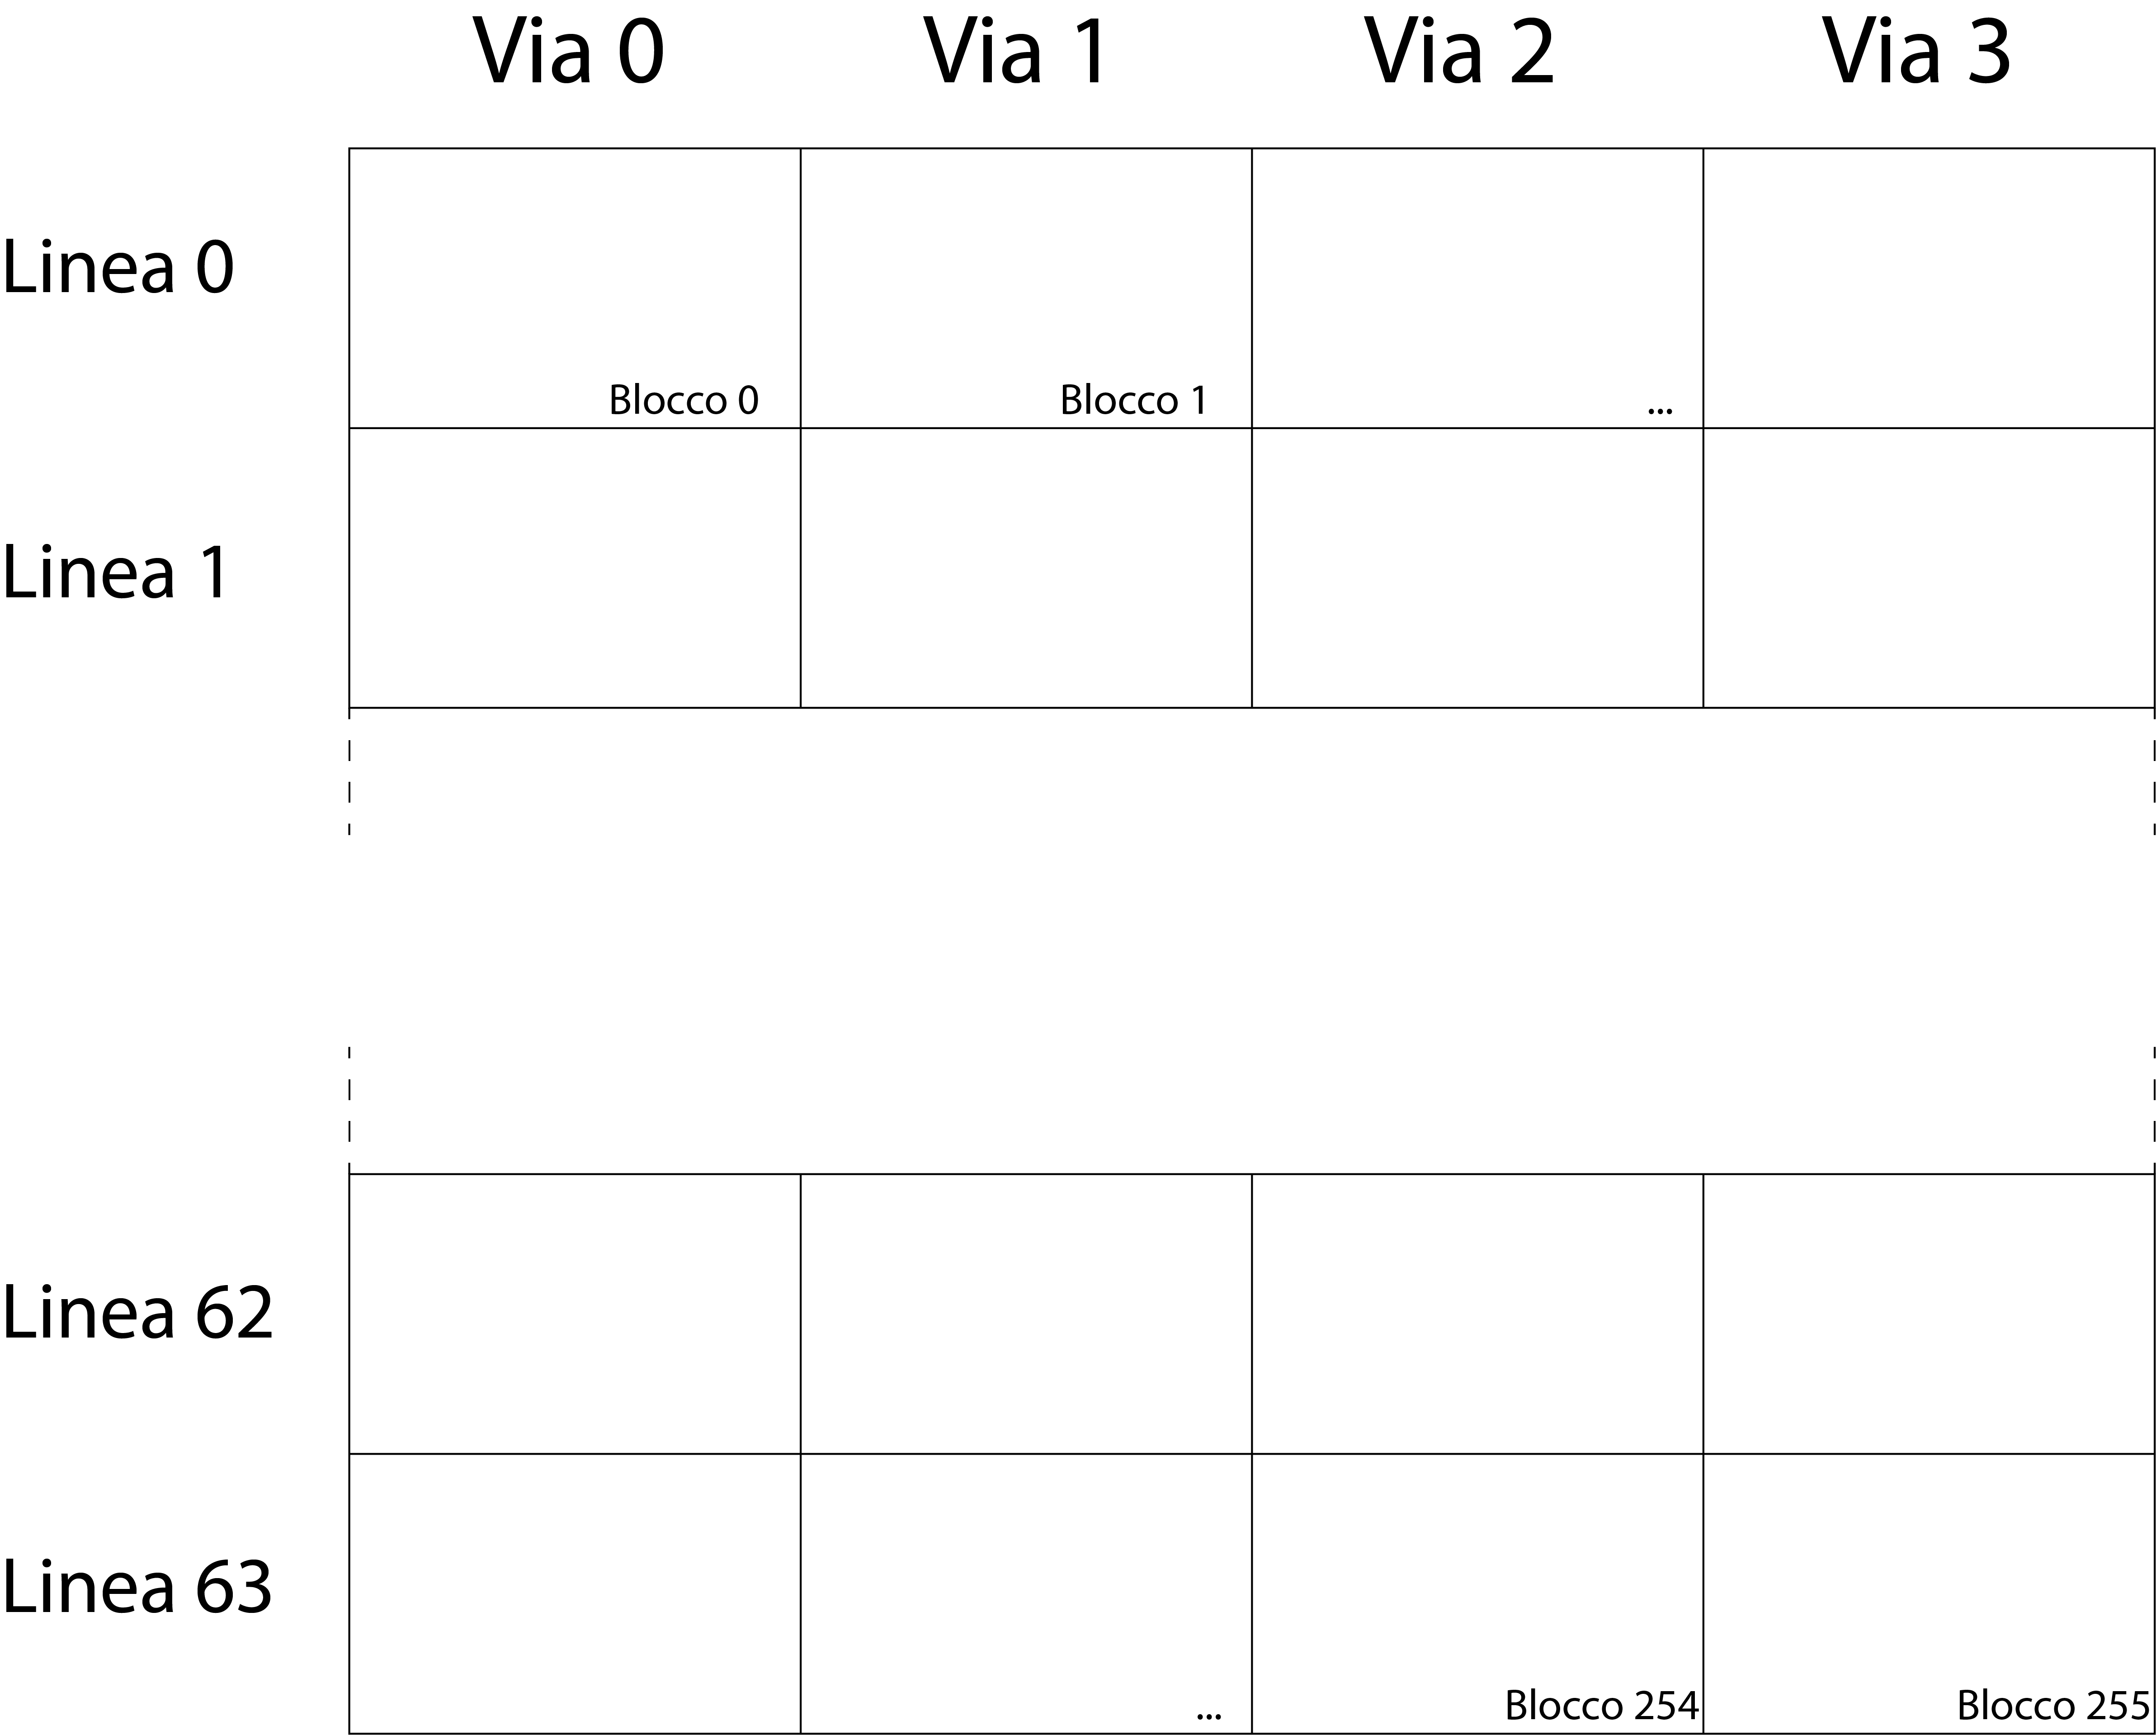
\includegraphics[width=.5\textwidth, keepaspectratio]{esempio-associativa}
\end{figure}
Ora è spiegato come viene memorizzato in cache un blocco di memoria.

Ad ogni blocco nella memoria centrale viene associata una linea con lo stesso meccanismo con cui in una cache a mappatura diretta si associa un blocco in cache.

Una volta che si identifica la linea a cui il blocco di memoria appartiene esso può essere memorizzato in uno qualsiasi dei blocchi di cache che compongono quella linea. Questo ci permette di avere in cache allo stesso momento due elementi che non sarebbero potuti essere compresenti in una cache a mappatura diretta.

Tuttavia dato che il numero di posizioni (nella cache) possibili per un blocco è ridotto (è lo stesso numero delle vie) l'implementazione risulta molto più semplice rispetto ad una cache completamente associativa.

\section{Mappatura del blocco}
In una cache a mappatura diretta abbiamo già osservato come un blocco di memoria centrale venga mappato in un blocco di cache deciso dalla formula:
\begin{equation*}
	\textrm{Indirizzo blocco} \pmod{\textrm{Numero blocchi della cache}}
\end{equation*}

In maniera simile in una cache set-associativa un blocco di memoria viene mappato in una \emph{linea} data da:
\begin{equation*}
	\textrm{Indirizzo blocco} \pmod{\textrm{Numero linee della cache}}
\end{equation*}
Quindi, per trovare il blocco all’interno della linea dobbiamo confrontare, in parallelo, il tag del blocco con tutti i tag dei blocchi di quella linea.

È ora inserito anche uno schema rappresentativo di una cache a 4 vie in cui ogni blocco contiene una word.

\begin{figure}[H]
	\centering
	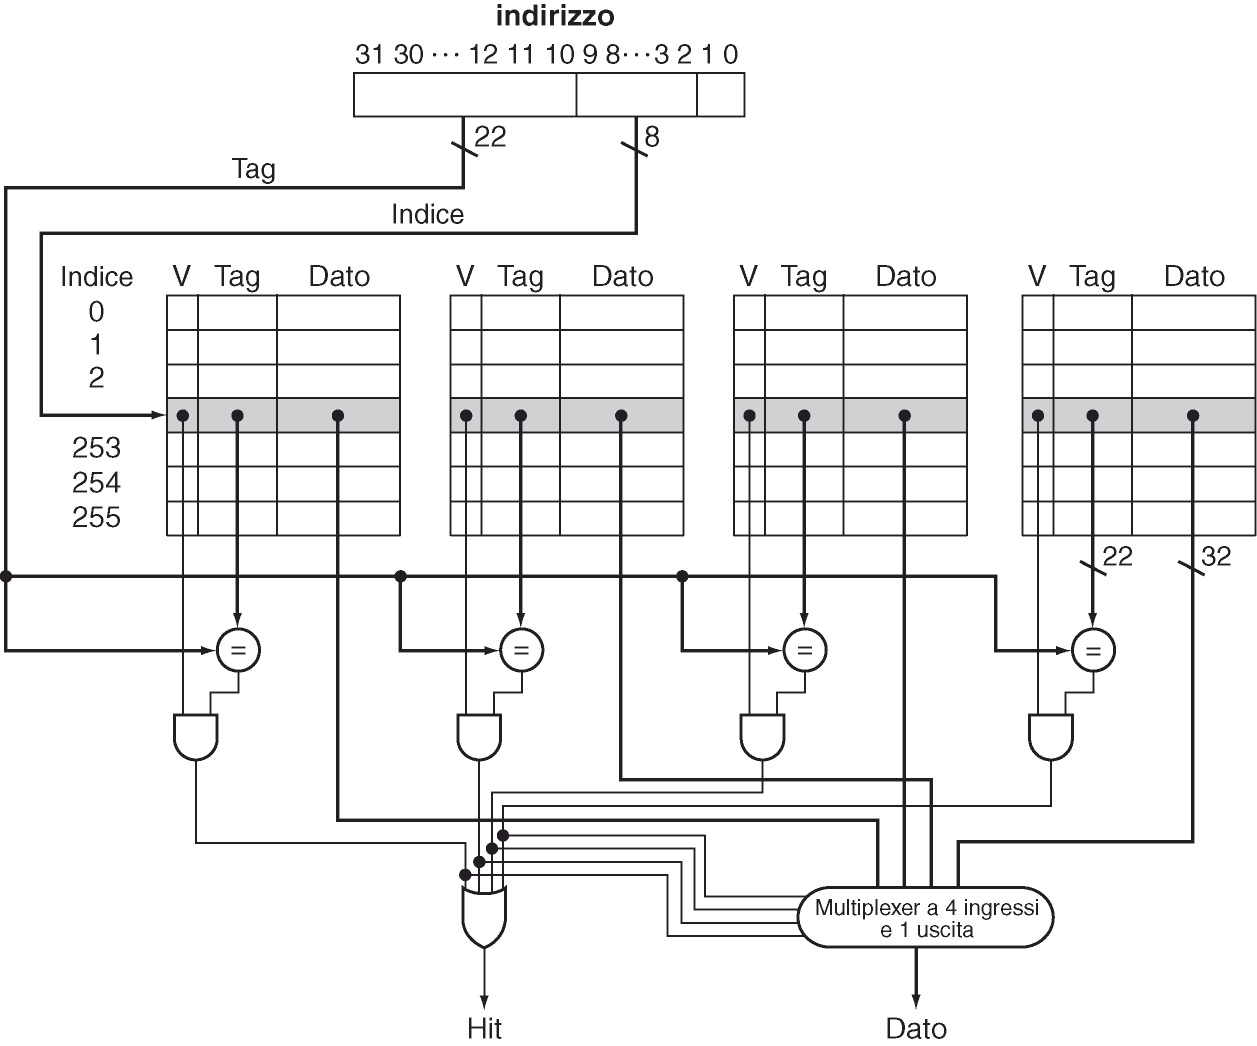
\includegraphics[width=0.8\textwidth,keepaspectratio]{4-vie}
\end{figure}
A seguire una breve descrizione dello schema.

I primi due bit dell'indirizzo (a destra) sono utilizzati per indicare, se necessario, quale singolo byte della word prelevare (sono due appunto perchè rappresentano i 4 possibili byte contenuti dal blocco).

Dato che le linee possibili sono 256 i bit che servono per rappresentarle sono 8, per l'appunto sono i bit dal 2 al 9 dell'indirizzo che vengono utilizzati come indicizzatore della linea (sia per la scrittura che per la lettura).

I bit rimanenti vengono utilizzati come tag del blocco; si noti che il tag viene confrontato con tutti e quattro i tag che ritornano dalle 4 vie.
Se il confronto va a buon fine vuol dire che il dato cercato è presente nella cache ed il mux a 4 ingressi si occupa di trasmetterlo al processore.

\section{Vantaggi dell'associatività}
Anche in questo caso è chiaro che la tecnologia che abbiamo trattato presenta vantaggi e svantaggi, è dunque giunto il momento di riassumerli e schematizzarli.
\begin{itemize}
	\item Vantaggi: aumentando l’associatività abbiamo il grosso vantaggio di diminuire la frequenza di miss e velocizzare il processo di reperimento dei dati.
	\item Svantaggi: purtroppo con questa implementazione la complessità dell'hardware aumenta in proporzione lineare al numero di blocchi della cache, ed allo stesso modo aumenta il costo.
\end{itemize}
Esiste inoltre un ulteriore problema che non abbiamo trattato: nelle cache a mappatura diretta, nel momento in cui si riscontra una cache miss, sicuramente è possibile conoscere chi sostituire, ossia l’unico blocco in cui è possibile mappare il dato che cerco. Nelle cache associative invece ci sono più scelte, quindi se la linea è piena chi bisogna sostituire? In tal caso esistono vari approcci possibili, tra cui:
\begin{itemize}
	\item \emph{FIFO}, un immancabile classico;
	\item \emph{LeastRecentlyUsed}, un metodo più sofisticato che però richiede una serie di bit in più per calcolare quando è avvenuto l'ultimo accesso.
\end{itemize}
Per concludere proponiamo al lettore anche un esempio pratico in cui si nota l'importanza della scelta di un buon meccanismo di cache mapping.
\begin{wrapfigure}{l}{0.55\textwidth}
	\centering
	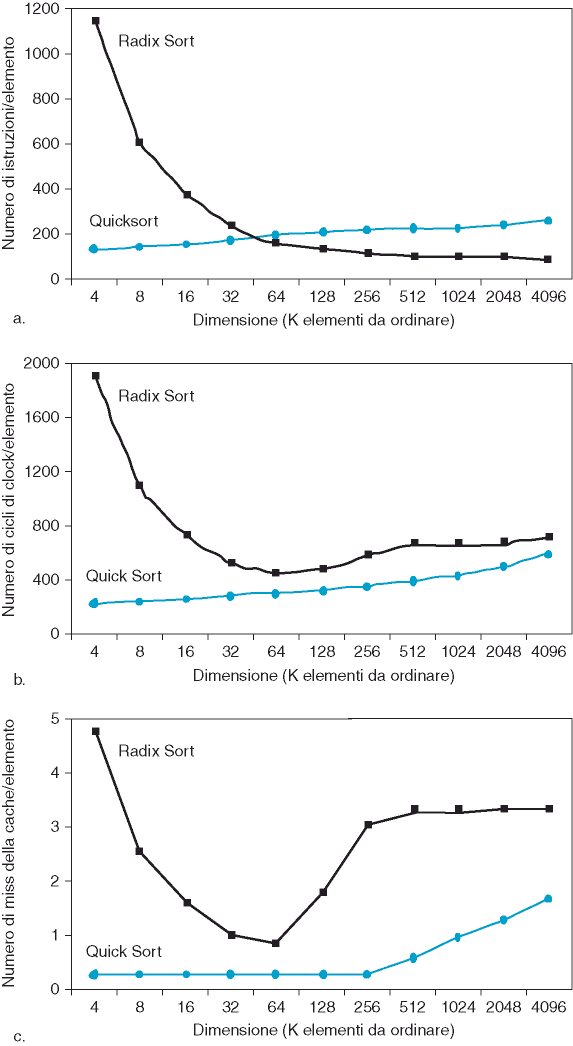
\includegraphics[width=0.7\linewidth,keepaspectratio]{grafici}
	\caption{Grafici prestazioni dei due algoritmi radix e quick sort}
\end{wrapfigure}
Si noti come nel primo grafico sembrerebbe che il radix sort sia asintoticamente più efficiente del quick sort, in quanto il suo rapporto
\begin{equation*}
	\frac{\textrm{numero di istruzioni}}{\textrm{elemento}}
\end{equation*}
scende molto sotto quello del quick sort.

Tuttavia nel secondo grafico si nota stranamente che il rapporto
\begin{equation*}
	\frac{\textrm{numero di cicli di clock}}{\textrm{elemento}}
\end{equation*}
del radix sort rimanga sempre più alto di quello del quick sort, decretando il radix sort come algoritmo più lento.

Nel terzo ed ultimo grafico si nota il perché di questa situazione anomala: il radix sort, per come è implementato, comporta un numero assai maggiore di miss della cache per ogni elemento che tratta e questo lo porta a ripetere perdere molti cicli di clock e quindi a risultare più lento.

\end{document}
